\colorlet{shadecolor}{\chapterColor}
\chapter{Armageddon}\label{a:Armageddon}
\markboth{\color{white}Armageddon \protect\thepage \hspace{4pt}}{}
\lhead{\textcolor{\chapterColor}{\rule[-2pt]{\textwidth}{15pt}}}
\qrcode{./maps/qr/Armageddon_qr.png}{http://maps.google.com/maps?q=44.43959094940084,-122.58215256842753}{Navigate to this area}
Located about 3.2 miles down quatzville road from highway 20, park in the Gravel pull out where the road bends about 0.1 miles before you reach a turnoff to a gravel road (which leads to the boulders). This area is also known as the upper garden. The lack of shade, the blackberries, the poison oak, and the 3 minute approach all make this area less desirable and less traveled then the Main
\begin{figure}[h]
  \centering
    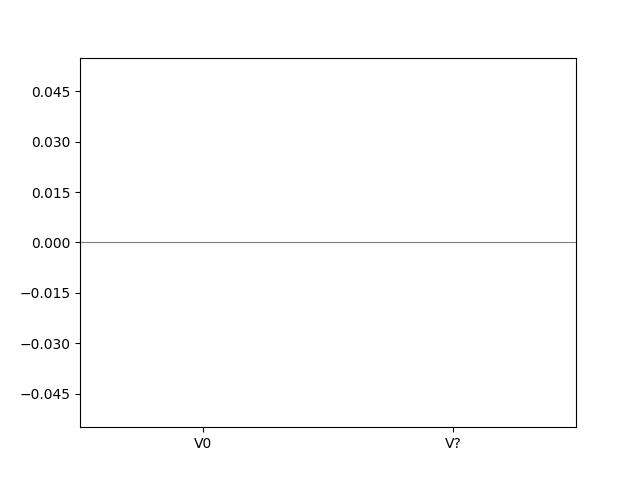
\includegraphics[width=\linewidth]{./maps/plots/Armageddon.png}
\end{figure}

\section{Entrance Area}\label{sa:Entrance Area}
\
\subsection*{Intro Boulder}\label{bf:Intro Boulder}
\

\section{The Bread Loaves}\label{sa:The Bread Loaves}
\
\subsection*{Lower Bread Loaf}\label{bf:Lower Bread Loaf}
\

\subsection*{Upper Bread Loaf}\label{bf:Upper Bread Loaf}
\

\section{Dr. Strangelove Area}\label{sa:Dr. Strangelove Area}
\
\subsection*{Dr. Strange Love}\label{bf:Dr. Strange Love}
\

\clearpage